% This section reframes agent context compression as sufficient-state approximation. The point is not to introduce a new optimization algorithm, but to state the objective that existing methods only approximate: the shortest representation that still supports future action.
% \begin{figure*}[ht]
%     \centering
%     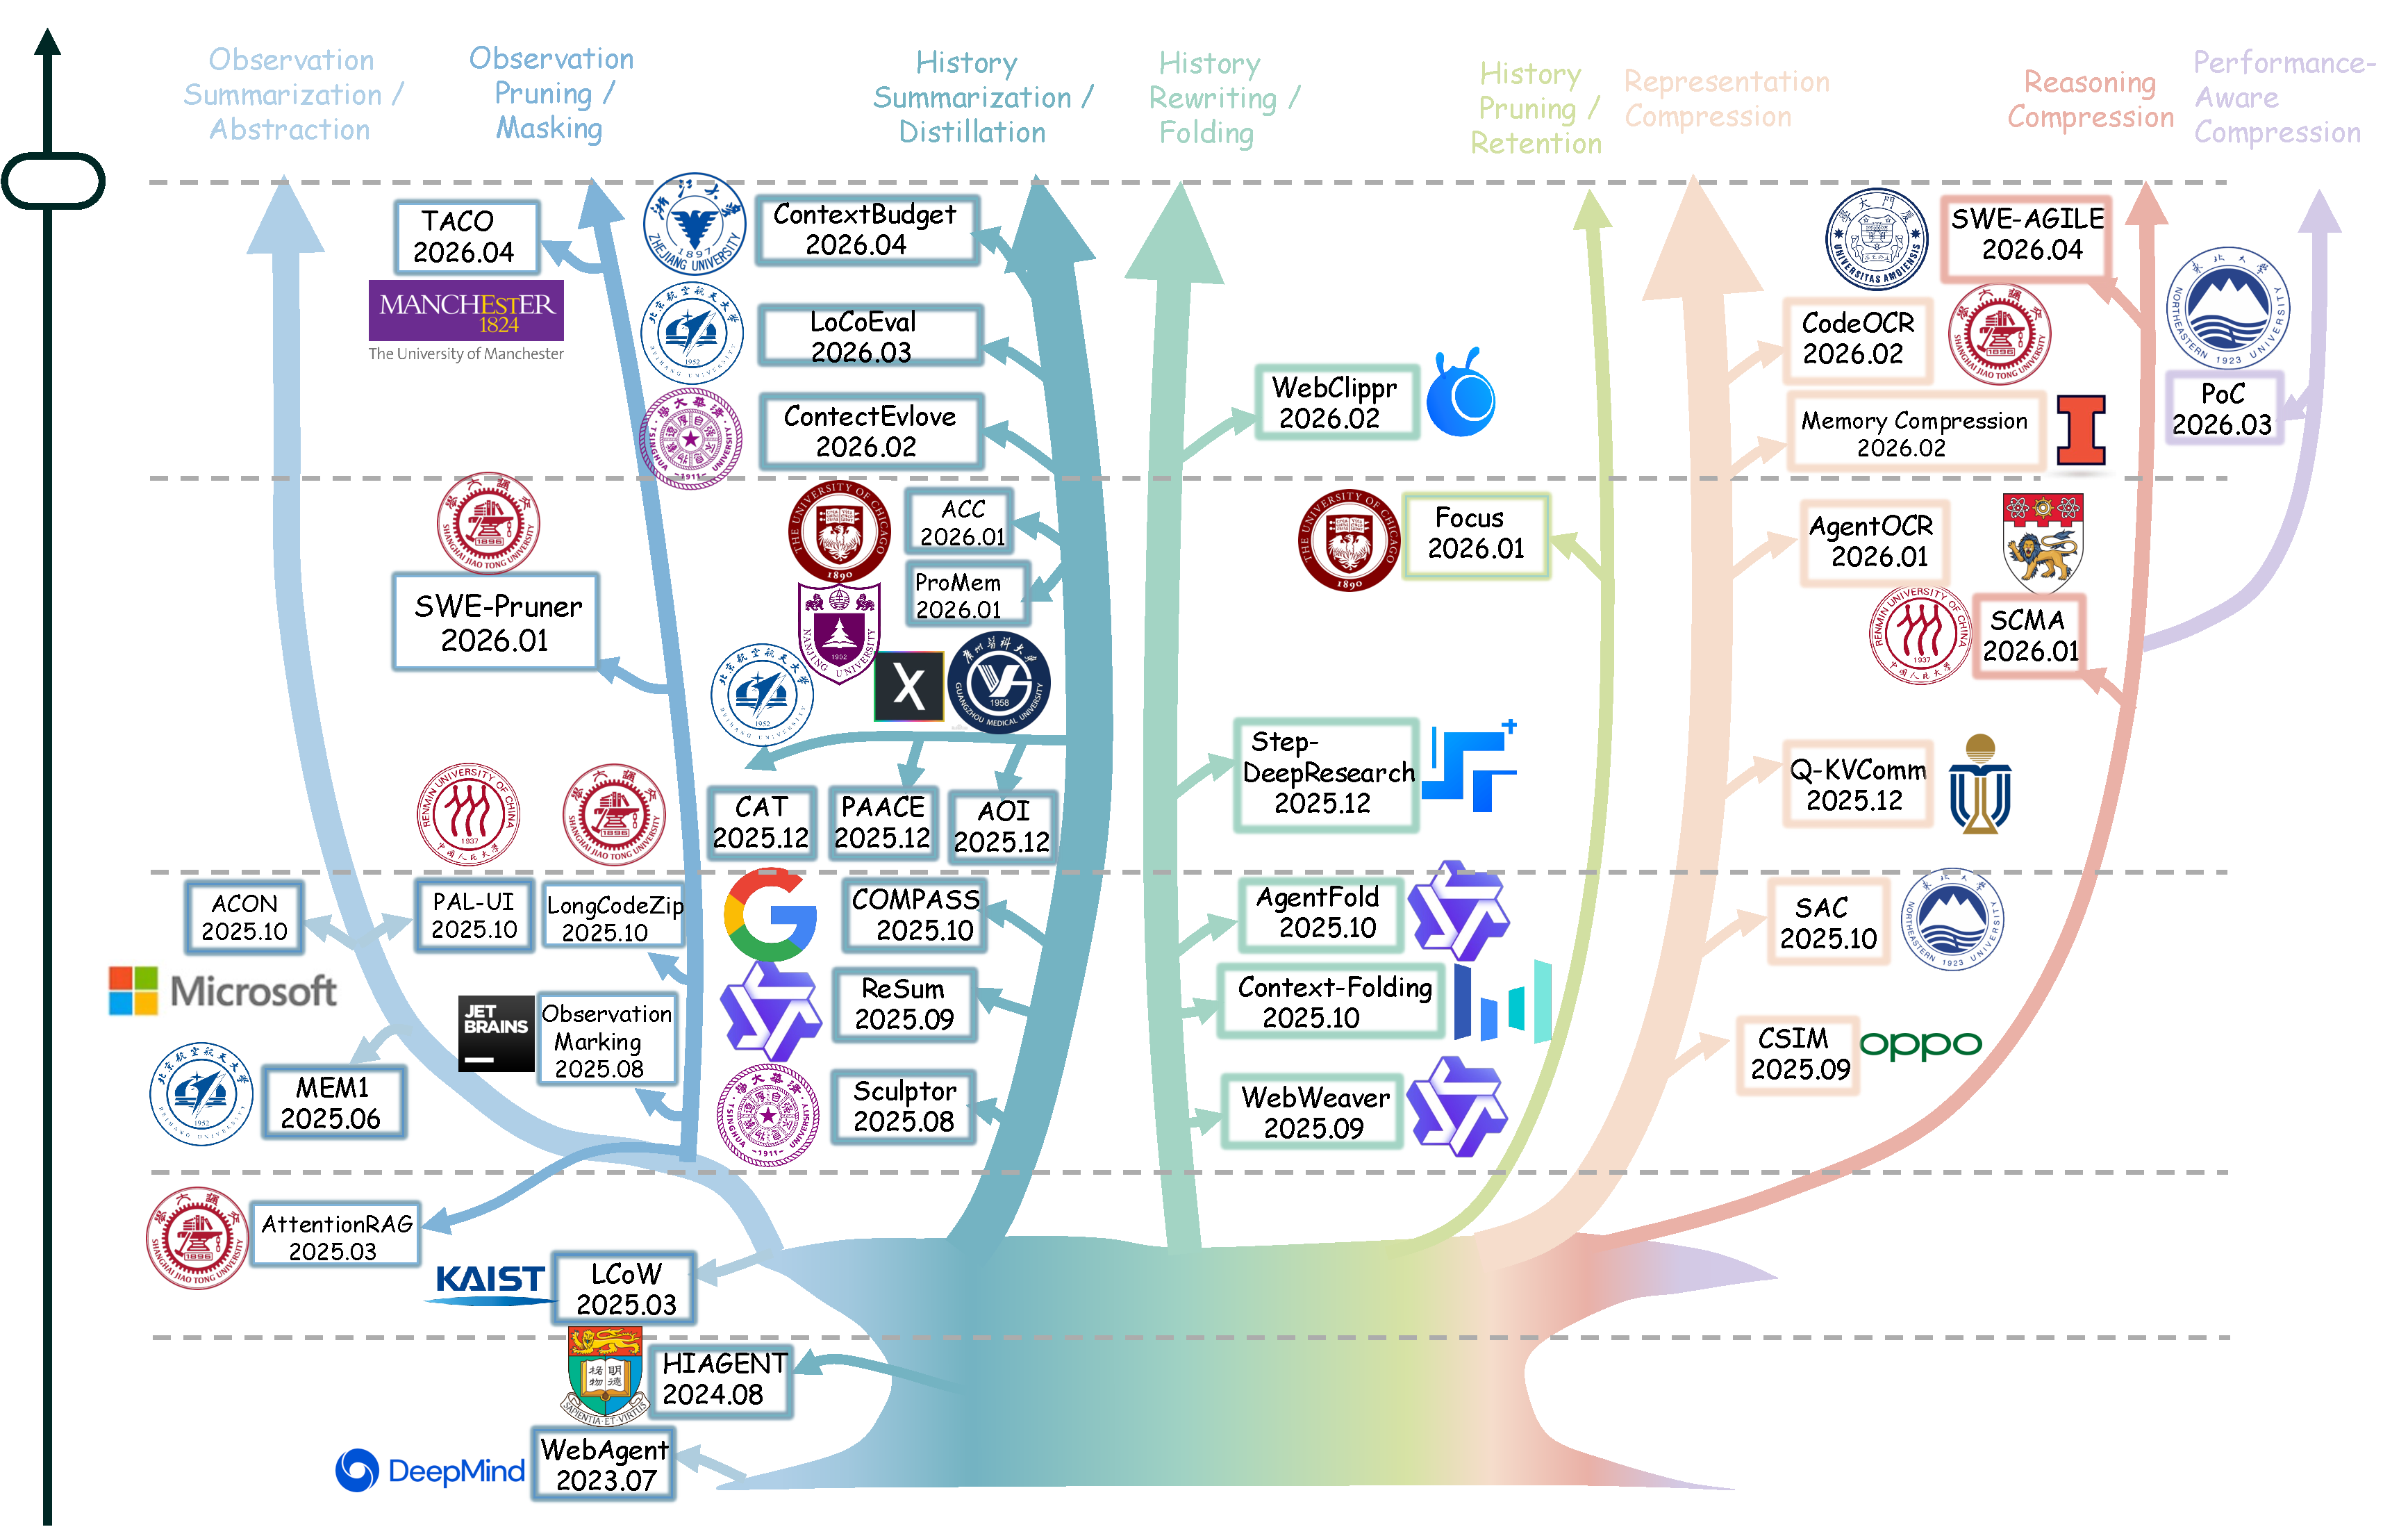
\includegraphics[width=0.74\textwidth]{figures/taxonomy.pdf}
%     \vspace{-.2cm}
%     \caption{A design-space view of agent context compression. The figure synthesizes targets, mechanisms, and control policies into a method-level landscape, grouping approaches by compression semantics while preserving chronological evolution. See Appendix~\ref{app:methodology} and \ref{ap:extended_taxonomies} for methodology, taxonomy details, and open-source resources.}
%     \label{fig:taxonomy_tree}
% \vspace{-.4cm}
% \end{figure*}

We argue that agent context compression is best understood as a sufficient-state approximation problem: the goal is to maintain the shortest representation that remains sufficient for future action.

\paragraph{Compression as State Transformation.} Let \(C_t\) denote the current context state. We treat each compression method as a transformation
{\setlength{\abovedisplayskip}{4pt}
\setlength{\belowdisplayskip}{4pt}
\setlength{\abovedisplayshortskip}{2pt}
\setlength{\belowdisplayshortskip}{2pt}
\[
O_i : \mathcal{C} \rightarrow \mathcal{C}, \qquad C_t' = O_i(C_t),
\]
}
where \(O_i\) maps \(C_t\) to a shorter, reorganized, or externally mediated representation \(C_t'\) under task-specific constraints. This abstraction is deliberately broad. It covers the operator families discussed later in the survey, including truncation, pruning, summarization, externalization, and representation-level compression.


\paragraph{Ideal Sufficient Memory.} From an algorithmic-information perspective, these operators can be viewed as practical approximations to an ideal sufficient memory. Let \(E_t\) denote the currently accessible environment state, \(A\) the agent policy or executor, \(\tau\) the task or task distribution, and \(\epsilon\) the maximum acceptable degradation in downstream performance. We define the ideal sufficient memory length as
\vspace{-.2cm}
\begin{equation}
\label{eq:ideal_sufficient_memory}
\begin{aligned}
L_{\epsilon}(C_t)
=
\min_{\tilde C_t \in \mathcal{S}_t}
&\ K(\tilde C_t \mid E_t) \\
\mathrm{s.t.}\quad
&\Delta_{\tau}(A; C_t,\tilde C_t,E_t) \leq \epsilon ,
\end{aligned}
\end{equation}
\vspace{-.1cm}
where \(\mathcal{S}_t = \mathcal{S}(C_t,E_t)\) denotes the admissible space of compressed states derived from \(C_t\) under environment \(E_t\). Here \(K(\tilde C_t \mid E_t)\) is standard conditional Kolmogorov complexity, and \(\Delta_{\tau}(A; C_t,\tilde C_t,E_t)\) measures the loss in future task performance induced by replacing \(C_t\) with \(\tilde C_t\). The quantity \(L_{\epsilon}\) is not meant as a computable training objective; rather, it serves as a stylized lower bound. A compressed state is useful only insofar as it remains compact, task-sufficient, and recoverable for future decisions.

\paragraph{From Approximation to Failure.} This objective turns the next two sections into one question: how does a method approximate a sufficient future state, and where can that approximation fail? Truncation bets that dropped spans have no future value. Pruning preserves an exact sufficient subset. Summarization replaces evidence with an executable abstraction. Externalization keeps part of the sufficient state off-context and shifts the bottleneck to recovery. Representation-level compression pushes sufficiency into latent space and sacrifices transparency. Under this view, the taxonomy compares approximation strategies, while the failure modes identify where sufficiency or recoverability is lost.

